% LaTeX Template for the reports in the B.Sc. Pharmaceutical Sciences
% Use XeLaTeX as the compiler
% Use XeLaTeX as the compiler
% Also check out the sample R-Script below! It makes your plotting easier
% GitHub from Jun Yin: https://github.com/jun0336/3rd_year_labs_ITpackage
\documentclass[12pt]{article}
\usepackage[utf8]{inputenc}
\usepackage{preamble} % 'preamble.sty' should be in the same folder

\begin{document}

\begin{titlepage}
\thispagestyle{firstpage}
\begin{center}
	\vspace*{.8cm}
    {\huge A \LaTeX Template for your report}
    \vskip 1cm
    {\large Group XXX\\
    B.Sc. Pharmaceutical Sciences, D-CHAB, ETH Zurich\\
    Vladimir-Prelog-Weg 1-5/10, 8093 Zurich, Switzerland\\}
    \vskip 0.5 cm
    {\begin{tabular}{ll}
    Student 1 & \href{mailto:student1@student.ethz.ch}{\textit{student1@student.ethz.ch}}\\
    Student 2 & \href{mailto:student2@student.ethz.ch}{\textit{student2@student.ethz.ch}}\\    
    Student 3 & \href{mailto:student3@student.ethz.ch}{\textit{student3@student.ethz.ch}}\\  
    \end{tabular}
    }
    
    \vskip .5cm
Assistant: 
\end{center}


\vskip 1 cm

\begin{abstract}

\end{abstract}

\vfill
\begin{center}

Z\"urich,  \today
\vskip 1.5 cm
\hskip 0 cm
\begingroup
  \wildcard{Student 1}
  \hspace{0.25cm}
  \wildcard{Student 2}
  \hspace{0.25cm}
  \wildcard{Student 3}
\endgroup
\end{center}

\end{titlepage}
\section{Introduction}


% Example of a scheme
\begin{scheme}[H]
    \centering
    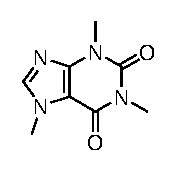
\includegraphics[scale=1]{coffein.eps} % You may alter the size
    \caption{Coffein}
    \label{coffein}
\end{scheme}

\section{Materials and Methods}
\subsection{Materials}


\subsection{Methods}


\section{Results}

\subsection{Determination of the protein concentration}

% Example of a figure
\begin{figure}[H]
    \centering
    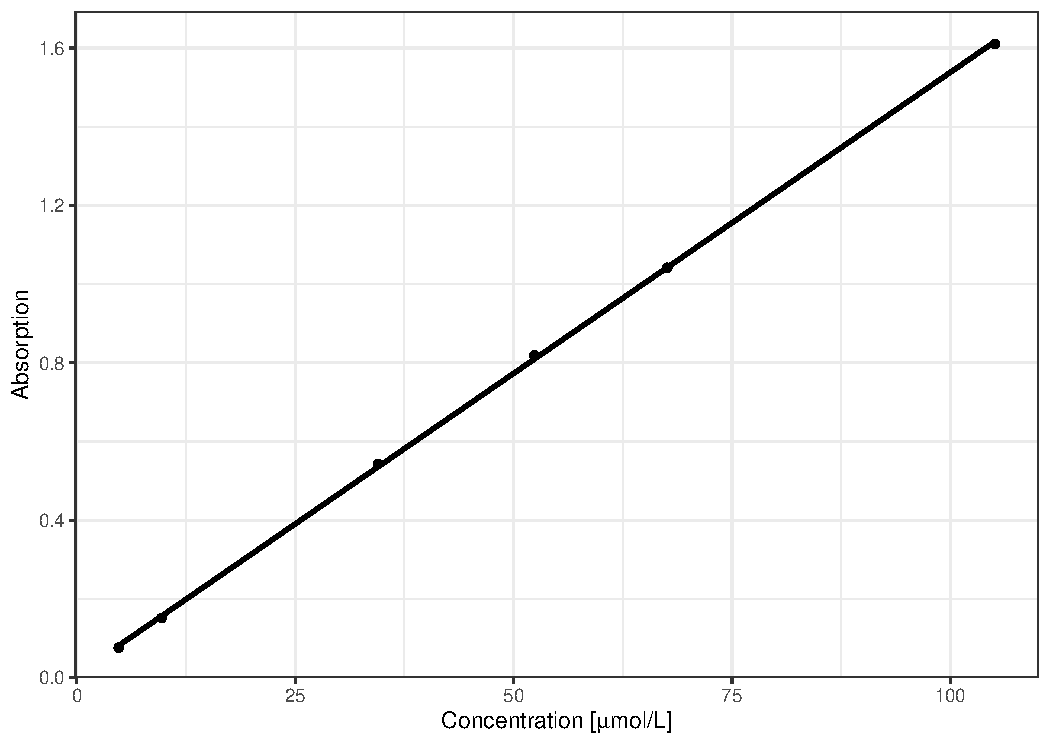
\includegraphics[scale=.5]{UVcurve.pdf}
    \caption{The UV calibration curve.}
    \label{biorad}
\end{figure}

% example of a table
\begin{table}[H]
\centering
\caption{The UV calibration curve is listed as a table.} 
\begin{tabular}{r|r}
  \toprule
Concentraion & Absorption \\ 
  \midrule
4.800 & 0.076 \\ 
  9.700 & 0.151 \\ 
  34.500 & 0.543 \\ 
  52.400 & 0.819 \\ 
  67.600 & 1.042 \\ 
  105.100 & 1.610 \\ 
   \bottomrule
\end{tabular}
\end{table}

\section{Discussion}

\section{Conclusion}

\printbibliography

\section*{Appendix}

\subsection*{Data}

\subsection*{R-Script}
\lstinputlisting[language=R]{Sample_RCode_UV.R}   
%\includepdf{eigen-vorlage.pdf}
\end{document}
